



% LLNCStmpl.tex
% Template file to use for LLNCS papers prepared in LaTeX
%websites for more information: http://www.springer.com
%http://www.springer.com/lncs
\documentclass{llncs}
\usepackage{graphicx}
%Use this line instead if you want to use running heads (i.e. headers on each page):
%\documentclass[runningheads]{llncs}
\begin{document}
\title{Edith}

%If you're using runningheads you can add an abreviated title for the running head on odd pages using the following
%\titlerunning{abreviated title goes here}
%and an alternative title for the table of contents:
%\toctitle{table of contents title}

\subtitle{Visual Editor}

%For a single author
%\author{Author Name}

%For multiple authors:
\author{Graham Baker, Walker Bohannan, Steve Marx, Vikram Nilakantan, \newline Jessica Penick and Eli Spiegel}


%If using runnningheads you can abbreviate the author name on even pages:
%\authorrunning{abbreviated author name}
%and you can change the author name in the table of contents
%\tocauthor{enhanced author name}

%For a single institute
%\institute{Institute Name \email{email address}}

% If authors are from different institutes 

\institute{University of Puget Sound}

%to remove your email just remove '\email{email address}'
% you can also remove the thanks footnote by removing '\thanks{Thank you to...}'


\maketitle

%\begin{abstract}
%abstract text goes here - Lorem ipsum dolor sit amet, consectetur adipiscing elit, sed do %eiusmod tempor incididunt ut labore et dolore magna aliqua.
%\end{abstract}

\clearpage

\section{Design Specification}

\subsection{Model-View Controller}
The architecture best for the visual editor module of Edith is the model-view-controller. This architecture, by splitting up the view controller and model into separate modules, allows us to separately tackle the issues of the draggable interface and the core structure of the editor. For example, a typical editor structure is a text box where the programmer might directly edit code, but given that code has special syntax, we could "cut the middle man" so to speak and provide the structures for the language with editable parts. This model also allows us to later adjust the interface to meet non-functional requirements like "easy to use."
 
\subsection{Alternatives}
Alternative architectures considered were the layered model and the pipe and filter model. The layered model also puts space between the interface and the core of the editor (the infrastructure layer) but the fact that each layer relies only on the layer beneath it is a kind of rigidity that will most likely hinder us later. Thus, this structure would make modifying the core editor module at later points in development more complicated than if each module was independent. The second alternative considered was the pipe and filter model, simply because it is a good structure for work flow. The model was rejected, however, because the scope of our module at this point is currently much narrower than document work flow. Our goal is to make a simple code editor and work our way into higher complexity from there. It is possible that we might later incorporate elements from these other models.

\subsection{UML Class Diagram}
\noindent\makebox[\textwidth]{%
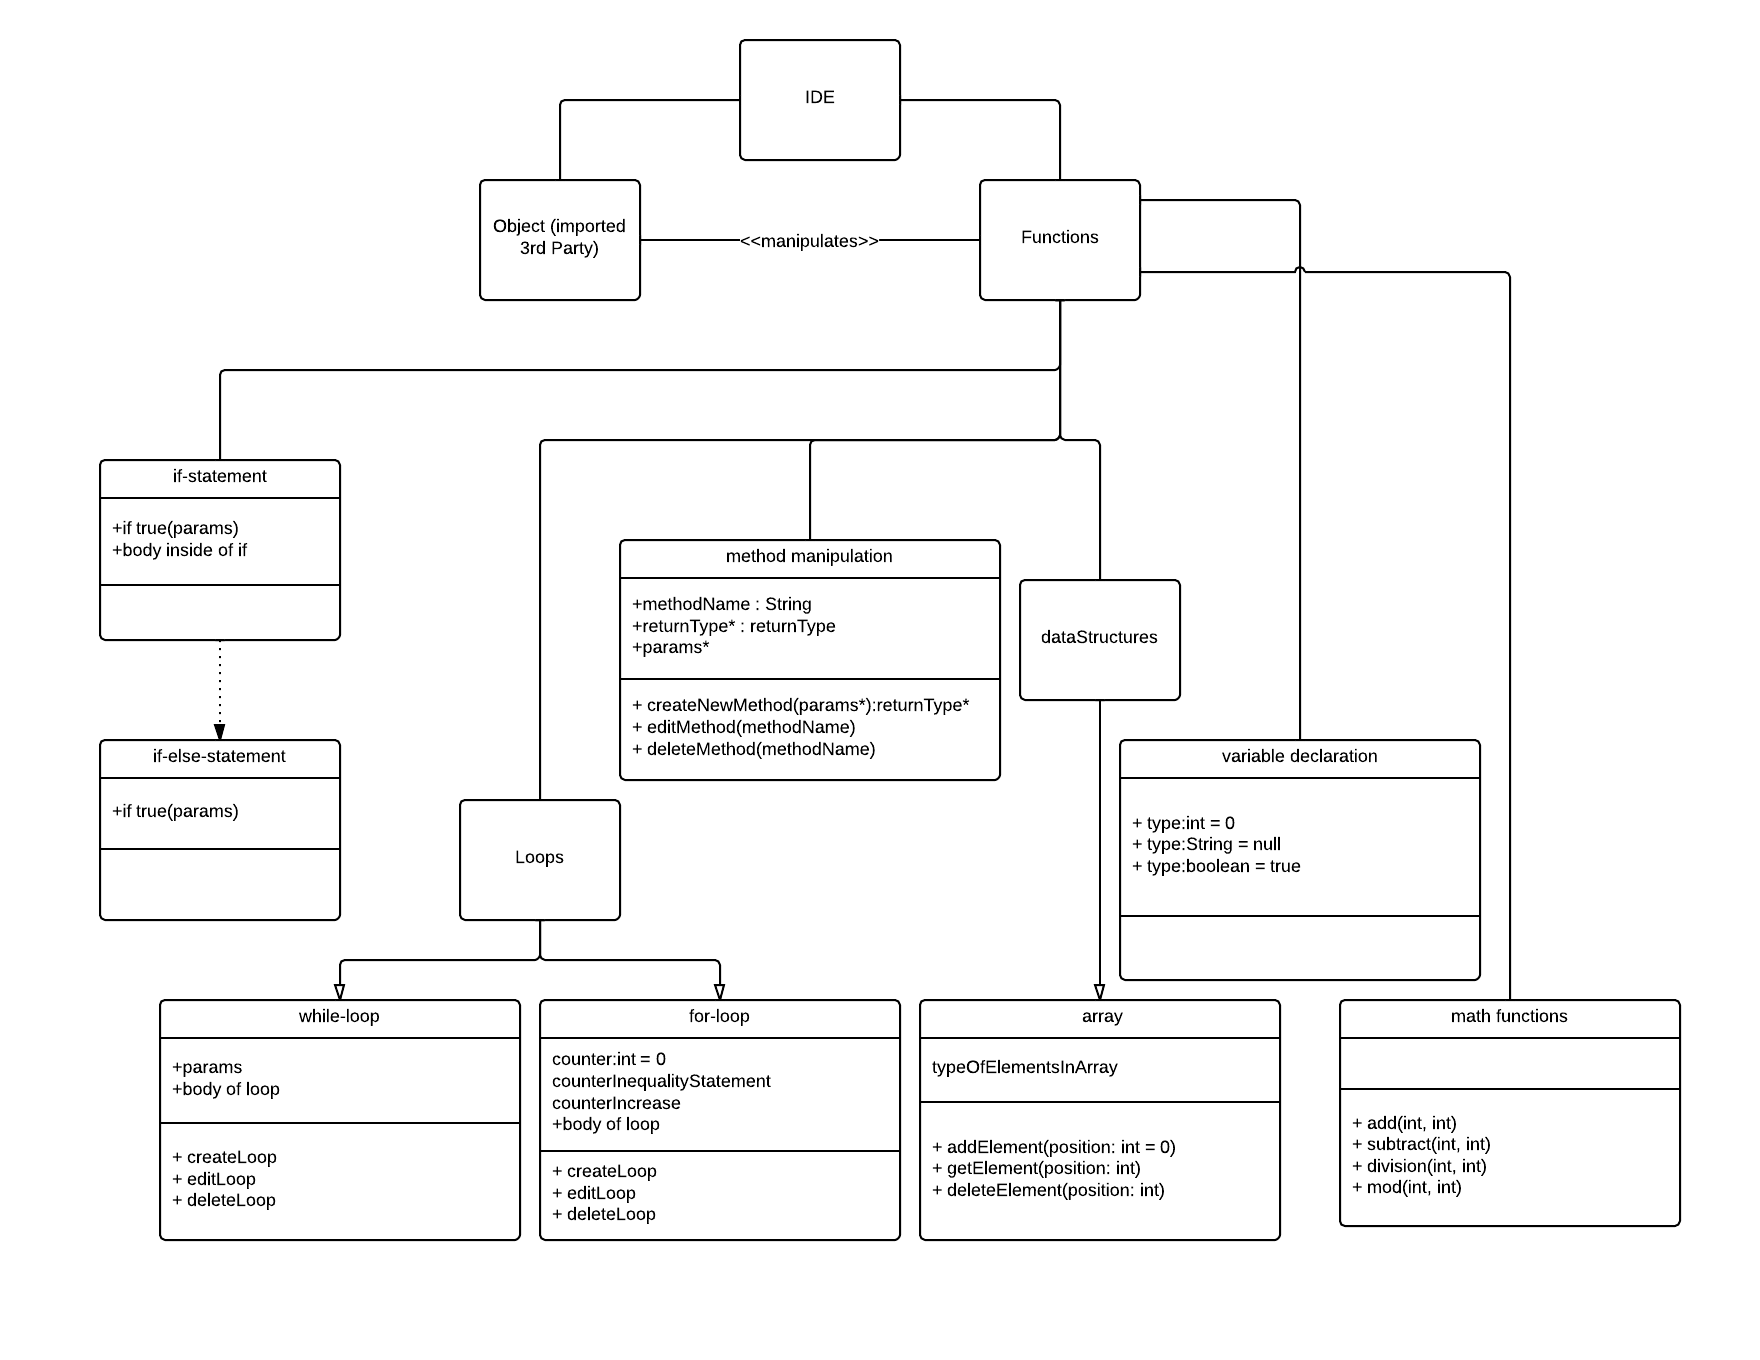
\includegraphics[width=1.8\textwidth]{visual_editor_uml.png}}

\clearpage

\subsection{User Interface Mock-Up}
\noindent\makebox[\textwidth]{%
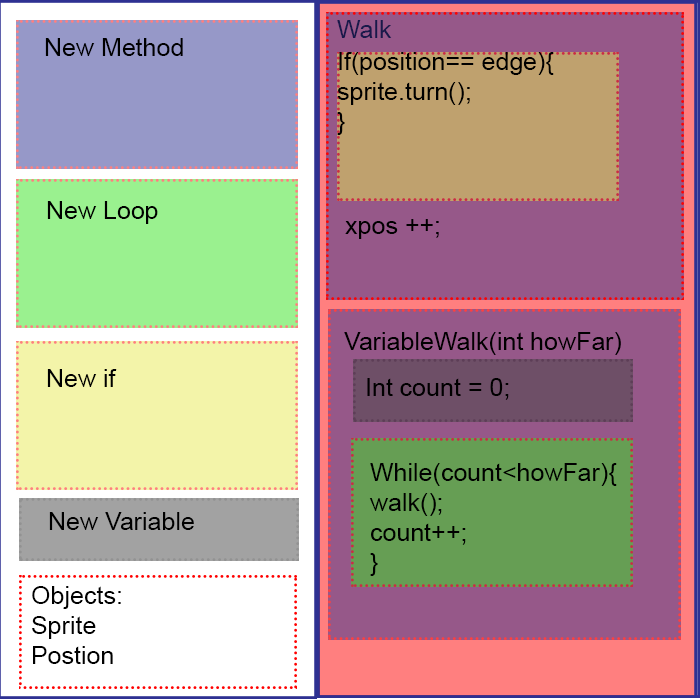
\includegraphics[width=1.0\textwidth]{UI.png}}

\clearpage

\section{Reflections and Status Update}

\subsection{Reflections on Development Process}
Developing a clear understanding of the Visual Editor’s role in the overall Edith project has been the major challenge.   Of course, it is easy to say that understanding the VE module’s role and its interaction with other modules should have been an easy first step.  However, even with somewhat detailed requirements specifications, some of the language can be interpreted in different ways, resulting in miscommunication.  

\subsubsection{}
On October 16 (two days before the submission deadline for this Intermediate Report), we learned that the VE team and another team understood their modules’ roles to be nearly identical - almost as if one of the teams thought it was the other team.  Most of the communication during development of the Requirements Specification was within the VE team or between the VE team and the professor.  Although the VE team communicated with other teams during work periods, the interactions were limited to a few questions and answers while teams figured out what their modules would do.  In retrospect, a more thorough review between teams whose modules interact would have been beneficial earlier in the design process.  Communication through the professor, as a third party and project client/designer, was important.  Some roles (e.g., method creation) for the final project remain unclear, but we are now more confident in the direction of VE development.  

\subsubsection{}
It seems that, early in the project, the team can most effectively tackle theoretical issues and make decisions on the development direction when meeting as a whole group.  As the project progresses, it may be beneficial to go through one segment of the work together as a team, particularly in cases where it could be used as a template.  As a small example, we created one or two use cases together before dividing the use cases among team members.  Coordination takes an investment of time up front, but can save later re-work and promote consistency.  Of course, as programming work increases, it will be divided among team members equitably (and considering interests and strengths).  

\subsubsection{}
In programming, as with anything, things take longer than expected. With a group of six people, it will be important to allow time for team member review and interaction as we approach milestones and deadlines.  This is some team members’ first experience writing software as part of a group (and being part of such a large software project).  Thus, some learning through trial and error is to be expected.


\subsection{Current Status Of Implementation}
\subsubsection{}
A thorough UML class diagram (included) has been developed.  Also, a mock-up of the Visual Editor’s user interface has been created, and the team will begin building toward that design. Given the confusion on the VE module’s role and its interaction with other modules (as described above), progress toward concrete build steps on the editor has been limited.  Now that the team has additional clarity, the build pace will need to increase to provide the first demonstration on November 1.  

\subsection{Timeline through Gantt Chart}
\subsubsection{}
\noindent\makebox[\textwidth]{%
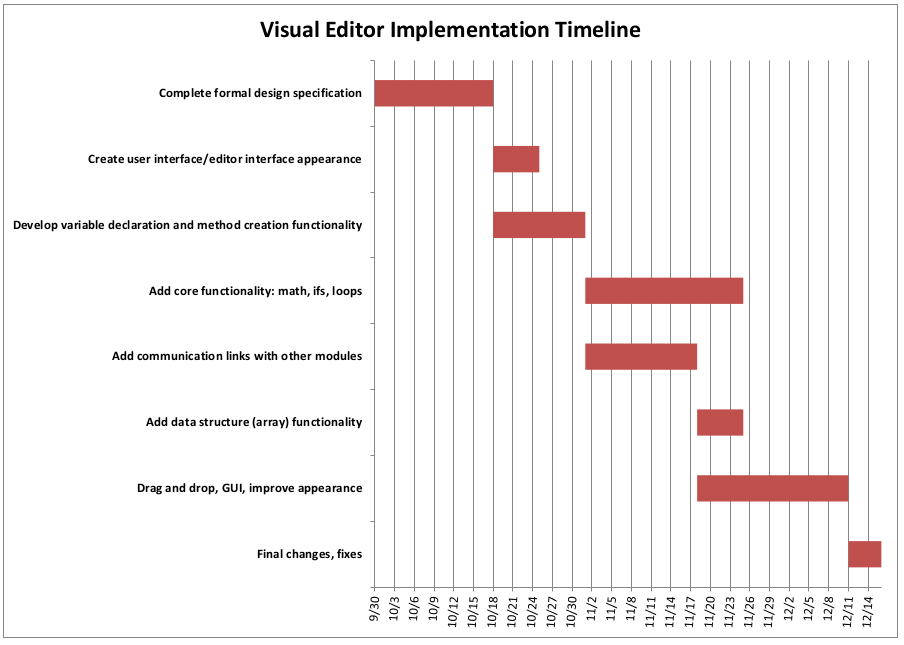
\includegraphics[width=1.0\textwidth]{gantt.png}}

\subsection{Team Member Responsibilities and Contributions}
\subsubsection{}We have done a good job of distributing work equitably and working together so far.  At this point, team members do not have assigned roles (e.g. GUI design, JSON specialist, etc.), and our work has consisted mainly of concept development and design.  Qualitatively, everyone has contributed and collaboratively worked toward the milestones (Requirements Specification and this Intermediate Report).  Quantitatively, call it 1/6 each.  Realistically, it is expected that not everyone will contribute exactly the same amount on each aspect of the program.  However, we do expect to contribute equally in total by the end of the project.  More specific roles will likely be assigned (at least for certain phases) as development pace increases.





%\begin{proposition}
%Insert proposition here
%\end{proposition}

%\begin{proof}
%Insert proof here
%\end{proof}

%The bibliography, done here without a bib file
%This is the old BibTeX style for use with llncs.cls
%\bibliographystyle{splncs}

%Alternative bibliography styles:
%the following does the same as above except with alphabetic sorting
%\bibliographystyle{splncs_srt}
%the following is the current LNCS BibTex with alphabetic sorting
%\bibliographystyle{splncs03}
%If you want to use a different BibTex style include [oribibl] in the document class line

%\begin{thebibliography}{1}
%add each reference in here like this:
%\bibitem[RE1]{reference1}
%Author:
%Article/Book:
%Other info: (date) page numbers.
%\end{thebibliography}

\end{document}

